\documentclass[main.tex]{subfiles}
\pagestyle{main}

\begin{document}
\chapter{Le cancer~: aspects biologiques et cliniques \label{chap:biologie_du_cancer}}%\todo[noline]{tumeur en general ou GIST?}
\mylettrine{L}{a} biologie du cancer est encore à ce jour non entièrement connue. 
Sa complexité n'étant pas des moindres, on présentera dans ce chapitre uniquement les points clés nécessaires à l'élaboration des modèles mathématiques présentés dans ce manuscrit (le lecteur pourra se référer à~\cite{bast2000tumor} pour une description détaillée de l'ensemble des phénomènes impliqués dans le cancer). 
Nous présenterons tout d'abord sommairement comment croît une tumeur, puis comment elle se répand dans l'organisme. Nous aborderons ensuite les traitements actuels. Puis nous examinerons de plus près le fonctionnement d'un scanner; les scanners constituant le seul et unique support d'informations médicales dont nous disposons. Enfin, la manière dont on évalue les réponses au traitement (le critère RECIST) sera présentée.

\section{Croissance tumorale}
%\todo[noline]{La tumeur en grandissant, va pousser vers l'extérieur le réseau sanguin qui l'alimente ! (La tumeur exerçant une pression sur celui-ci) --> valable que pour les méta, tumeur primit = infiltrante}
Une tumeur est un ensemble de cellules de l'organisme se multipliant de manière dégénérée. %\footnote{%Par dégénérée, on entend : autonome, agissant pour son propre compte.}. 
Certains scientifiques s'accordent à dire que cela partirait d'une seule cellule (bien que pour l'instant aucune preuve de cela n'a encore été apportée~: le sujet reste ouvert). 
Après la mitose, chaque cellule fille est alors à son tour dégénérée et se multiplie. %% encore et encore. 
Sans limitation, la tumeur pourrait alors grandir exponentiellement. 
En réalité, la croissance tumorale est limitée par les besoins en glucose et en oxygène. 
En effet, à force de se multiplier les cellules sont en surpopulation. 
%%Le réseau sanguin environnant ne suffit plus à subvenir aux besoins de la tumeur. 
Les nutriments et l'oxygène viennent à manquer : c'est l'\emph{hypoxie}. 
Les cellules du bord de la tumeur consomment ainsi tous les apports nutritifs amenés par le réseau sanguin environnant et n'en laissent pas assez pour celles situées plus au centre. 
C'est dans ces cas là que l'on peut voir sur les scanners des tumeurs avec deux nuances de gris~:
\begin{myitemize}
\item un gris foncé au centre, emplacement du tissu en partie nécrosé
\item un gris plus clair sur le pourtour, lieu de la prolifération
\end{myitemize}


%%%% Il faut faire un paragraphe pour que wrapfigure puisse se fixer
%%%% Pour ne pas que ca ait l'apparence d'un paragraphe, on peut supprimer l'indentation
%\begin{wrapfigure}[26]{R}{.62\textwidth}
\begin{wrapfigure}[26]{O}{.62\textwidth}
%%\vspace{-15mm}
\vspace{10mm}
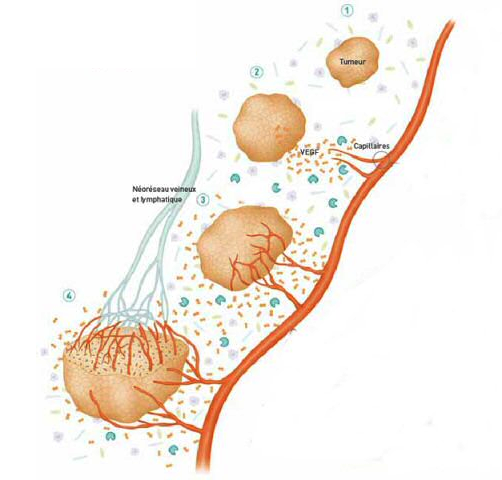
\includegraphics[width=.65\textwidth, trim= 17mm 0cm 1cm 0cm  , clip=true ]{schema/angiogenese.jpg}
\caption{\label{fig:schema_angio} Schéma descriptif de l'angiogénèse générant la néovascularisation \cite{webangiogenese}.}
\end{wrapfigure}
%\newpage


\paragraph{}
Les cellules en hypoxie vont alors entrer dans un état de quiescence et vont sécréter des \emph{facteurs de croissance}, dont le VEGF\footnote{de l'anglais~: Vascular Endothelial Growth Factor}. 
Ces protéines commandent la création de nouveaux vaisseaux  
 sanguins, processus appelé \emph{angiogenèse}. 
Les cellules endothéliales -- cellules qui recouvrent la paroi intérieure des vaisseaux sanguins -- sont les destinataires de ces facteurs de croissance. 
Elles possèdent des \emph{récepteurs} spécifiques au VEGF, les VEGFRs. 
Au contact du VEGF, les VEGFRs vont activer diverses fonctionnalités des cellules endothéliales comme leur division et leur maturation. 
Ceci fournit le matériel nécessaire à la création de nouveaux vaisseaux sanguins. 
Ils sont construit par \emph{chimiotactisme} \cad qu'ils sont 
 orientés dans le sens où la concentration de facteur de croissance est la plus forte. 
%%%%%%%%%%%%%%%%%%%%%%%%
%%%%Les cellules en hypoxie vont alors entrer dans un état de quiescence et vont sécréter des \emph{facteurs de croissance}, dont le VEGF (Vascular Endothelial Growth Factor). 
%%%%%%Ces molécules parviennent jusqu'aux récepteurs de VEGF (VEGFR) situés sur les cellules endothéliales,  cellules qui recouvrent la paroi intérieure des vaisseaux sanguins. 
%%%%\noindent
%%%%Ces protéines commandent la création de nouveaux vaisseaux  
%%%%\noindent
%%%%sanguins, processus appelé \emph{angiogenèse}. 
%%%%Les cellules endothéliales, cellules qui recouvrent la paroi intérieure des vaisseaux sanguins et destinataires de ces facteurs de croissance, vont alors se diviser et maturer afin de fournir le matériel nécessaire à la création de nouveaux vaisseaux sanguins. 
%%%%Ceux-ci sont construit par \emph{chimiotactisme} \cad qu'ils sont 
%%%% orientés dans le sens où la concentration de facteur de croissance est la plus forte. 
%%%%%%%%%%%%%%%%%%%%%%%


 
 Ainsi la tumeur se crée son propre réseau sanguin~: la \emph{néovascularisation}, comme représenté  sur la Figure~\ref{fig:schema_angio}. Les nutriments et l'oxygène redeviennent de nouveau abondants. 
Les cellules qui étaient en hypoxie vont alors se remettre à proliférer jusqu'à ce que de nouveau, il y ait surpopulation. Et ainsi de suite, le cycle continue. 
%%On peut visualiser ce cycle sur le schéma présenté Figure~\ref{fig:schema_angio}. 


Notons qu'une cellule saine se comporte de manière différente~: %%n'est en général jamais quiescente~: 
si les conditions extérieures ne sont pas bonnes (surpopulation, manque de nutriments, etc), elle va activer son auto-destruction~: c'est l'\emph{apoptose}. A cause de mutations, les cellules cancéreuses sont nettement moins (voire pas) sensibles à ce mécanisme. 
%\lipsum[1]

\newpage
\section{Dissémination des métastases}
\begin{wrapfigure}[18]{o}{.5\textwidth} %%% L : Left flottant / l: left non flottant (pas de pagebreak) o : oven (a l'exterieur)
\setlength{\unitlength}{.005\textwidth}
\vspace{-7mm}
\begin{picture}(100,93)
\tiny 
\put(0,2){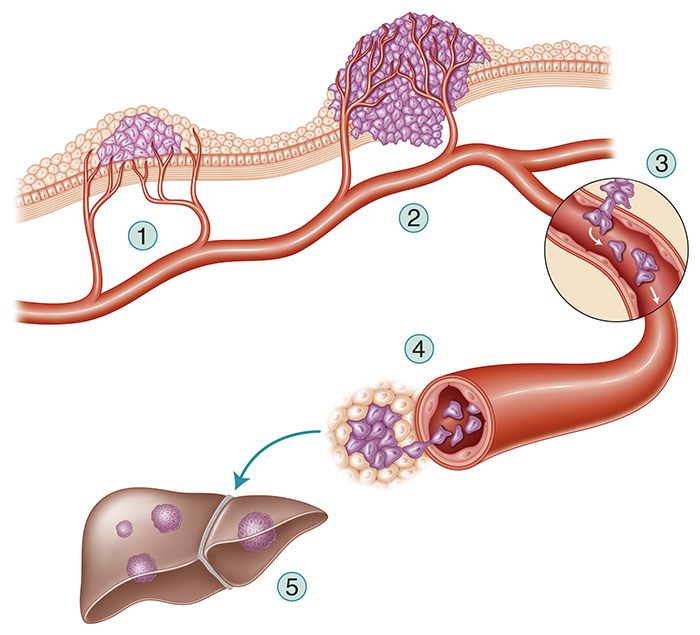
\includegraphics[width=.5\textwidth]{schema/cellules_tumorales_circulantes_copyright.jpg}}
\put(30,0){Copyright Eléonore Lamoglia/Institut Curie}
%%\put(0,0){\rect{0}{0}{100}{93}}
\end{picture}
\captionof{figure}{\label{fig:schema_dissemination_metastase} Dissémination des métastases.}
\end{wrapfigure}
L'ensemble du processus métastatique est résumé sur le schéma de la %%présenté 
 Figure~\ref{fig:schema_dissemination_metastase}. Décrivons-le. La tumeur primaire  cherche continuellement à se vasculariser davantage, %toujours plus, 
 mais paradoxalement, sa croissance va endommager le réseau sanguin qui l'irrigue. Une partie des cellules tumorales (cellules invasives) va alors pouvoir pénétrer dans les voies sanguines. La plupart de ces essaims seront éliminés par le système immunitaire. Une partie arrivera à s'installer dans un autre organe~: elle forme des tumeurs filles appelées~\emph{métastases}. Chaque type de cancer a une préférence métastatique~\cite{nguyen2009metastasis,langley2011seed}~: le GIST, le cancer du pancréas ou du colon migre au foie; les cancers du sein, du rein, de la vessie et de l'estomac migrent dans les poumons; le cancer de la prostate migre dans les os. Les métastases s'installent généralement dans des endroits bien vascularisés~:  les poumons et le foie sont les deux organes les plus touchés. %%\todo[REF].


De simples cellules ne pourraient pas nicher dans un autre organe que celui auquel elles appartenaient au départ. Les cellules tumorales le peuvent, car à force de divisions elles s'\emph{indifférencient}. Autrement dit, elles s'approchent de ce qu'elles étaient au stade embryonnaire~: des cellules souches qui en se différenciant formeront aussi bien des cellules de l'intestin que des cellules du foie. Dans le cas de métastases hépatiques en provenance de GIST, les cellules cancéreuses provenant de l'intestin ne sont donc pas reconnues comme étrangères au foie et la métastase peut s'installer. La métastase créera ensuite son propre réseau néovasculaire tout comme une tumeur primaire.

\section{Les traitements}
A l'heure actuelle aucun traitement ne permet de guérir de manière sûre les cancers, d'autant plus s'ils sont avancés. Cependant plusieurs techniques existent pour prolonger et/ou améliorer la vie des patients.
\paragraph{La chirurgie} ne peut-être réalisée que sur des cancers primaires %, non métastasés et donc 
détectés tôt. C'est la première option considérée par le corps médical (bien que la chirurgie elle-même puisse être source de dissémination de métastase, \cf par exemple~\cite{topal2005cancer}.

\paragraph{L'ablation par radiofréquence} (ou bien aussi la cryoablation, les micro-ondes et l'électroporation) permet, à l'aide d'une sonde électromagnétique à haute fréquence, de brûler une région définie par le médecin. Par ce biais, une ablation peut être effectuée sans avoir à opérer le patient. 
Cette technique ne peut cependant être utilisée que pour des petites tumeurs, ne dépassant pas une certaine taille (jusqu'à 6 centimètres maximum) et n'étant pas à proximité d'organes sensibles. 

\paragraph{La radiothérapie} consiste à irradier une zone de l'organisme par une forte dose de rayons X (et rayonnement bêta pour la curiethérapie). 
%Ceci produit des radicaux libres par radiolyse de l'eau, et donc altération de l'ADN. 
Ceci engendre une altération de l'ADN et permet de réintroduire de l'apoptose dans le cycle cellulaire. 
%Ceci a pour effet de détruire les cellules qui se multiplient et donc, par voie de conséquence, les cellules cancéreuses. 
%Cette méthode présente les mêmes limitations que la radiofréquence à savoir que son efficacité est limitée à des petites tumeurs. 
Cette méthode est également utilisée sur de petites (ou moyennes) tumeurs, car sur des tumeurs plus importantes, il y a des effets secondaires. 
La radiothérapie peut être %est souvent 
utilisée à titre palliatif sur des petites métastases (pulmonaires notamment).

\paragraph{Les chimiothérapies} regroupent un ensemble de médicaments \emph{cytotoxiques} (\ie qui détruisent les cellules) administrés en intraveineuse. 
%%Ce type de molécules est suffisamment petit pour pénétrer à l'intérieur des cellules. 
%% Elle agit 
Après avoir pénétré à l'intérieur des cellules, ce type de molécules agit 
sur toutes les cellules en division trop rapide en affectant soit directement la mitose, soit la duplication de l'ADN. 
Ceci explique ses principaux effets secondaires car elle va impacter aussi des cellules saines à division naturellement rapide comme les cellules responsables de la pousse des cheveux, les cellules intestinales (de l'épithélium), les cellules sanguines (à l'origine d'affaiblissements du système immunitaire et d'anémies notamment) ou encore les gamètes.

\paragraph{Les thérapies ciblées} sont des médicaments qui peuvent également être administrés par voies intraveineuses, mais sont de plus en plus prescrits en %métronomique sous forme de cachet à. Des versions
systémique 
%commencent également à voir le jour 
(\ie sous forme de comprimés à prendre à heures fixes). Bien qu'étant diffusées dans tout l'organisme, ces thérapies ciblent un type spécifique de voies moléculaires (ou de récepteurs), voies moléculaires généralement caractéristiques des cellules malignes. 
\correction{Chaque fonction cellulaire (mitose, apoptose, quiescence, ...) est régie par un ensemble de protéines qui agissent en cascade comme messagers~: les \emph{tyrosines kinases} (TK) (\cf Figure~\ref{fig:TK}). Les  thérapies ciblées inhibent ces tyrosines. Elles peuvent être des anticorps (le nom de la molécule thérapeutique est alors de la forme X-mab), comme illustrés sur la Figure~\ref{fig:TKI} ou de petites molécules ciblant les récepteurs de tyrosines kinases (RTK)  comme présentées sur la Figure~\ref{fig:RTKI} (le nom de la molécule est alors ici de la forme X-nib).}
%Ce peut être des anticorps (X-mab) ou de petites molécules ciblant les fonctions tyrosines kinases (X-inib), fonctions impliquées dans l'activité cellulaire et la mitose. 

\begin{figure}
\subfloat[\label{fig:TK}Les tyrosines kinases~: des messagers cellulaires]{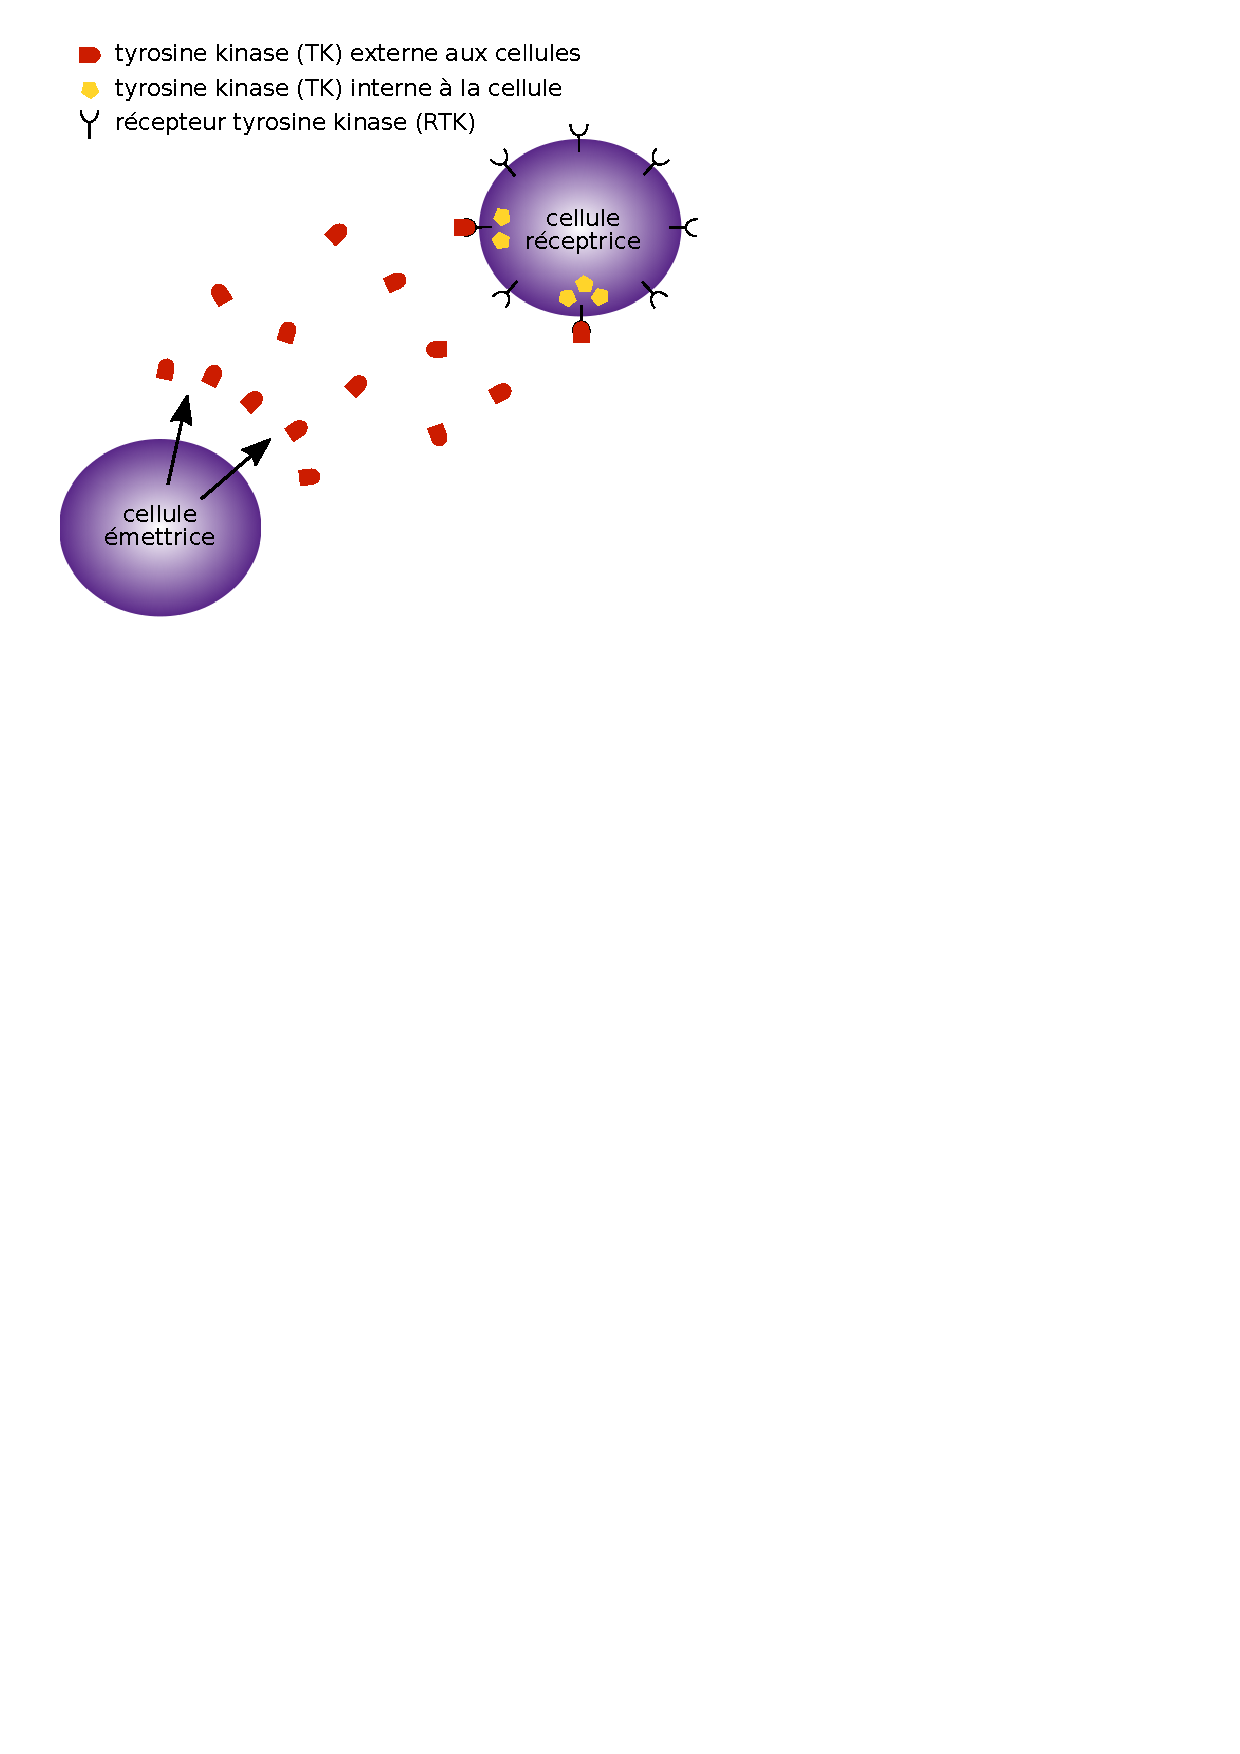
\includegraphics[trim= 0mm 190mm 85mm 0mm, clip=true, width=.32\textwidth]{schema/voies_moleculaires.pdf}}\hfill
\subfloat[\label{fig:TKI}Mode d'action d'un inhibiteur de tyrosine kinase (X-mab)]{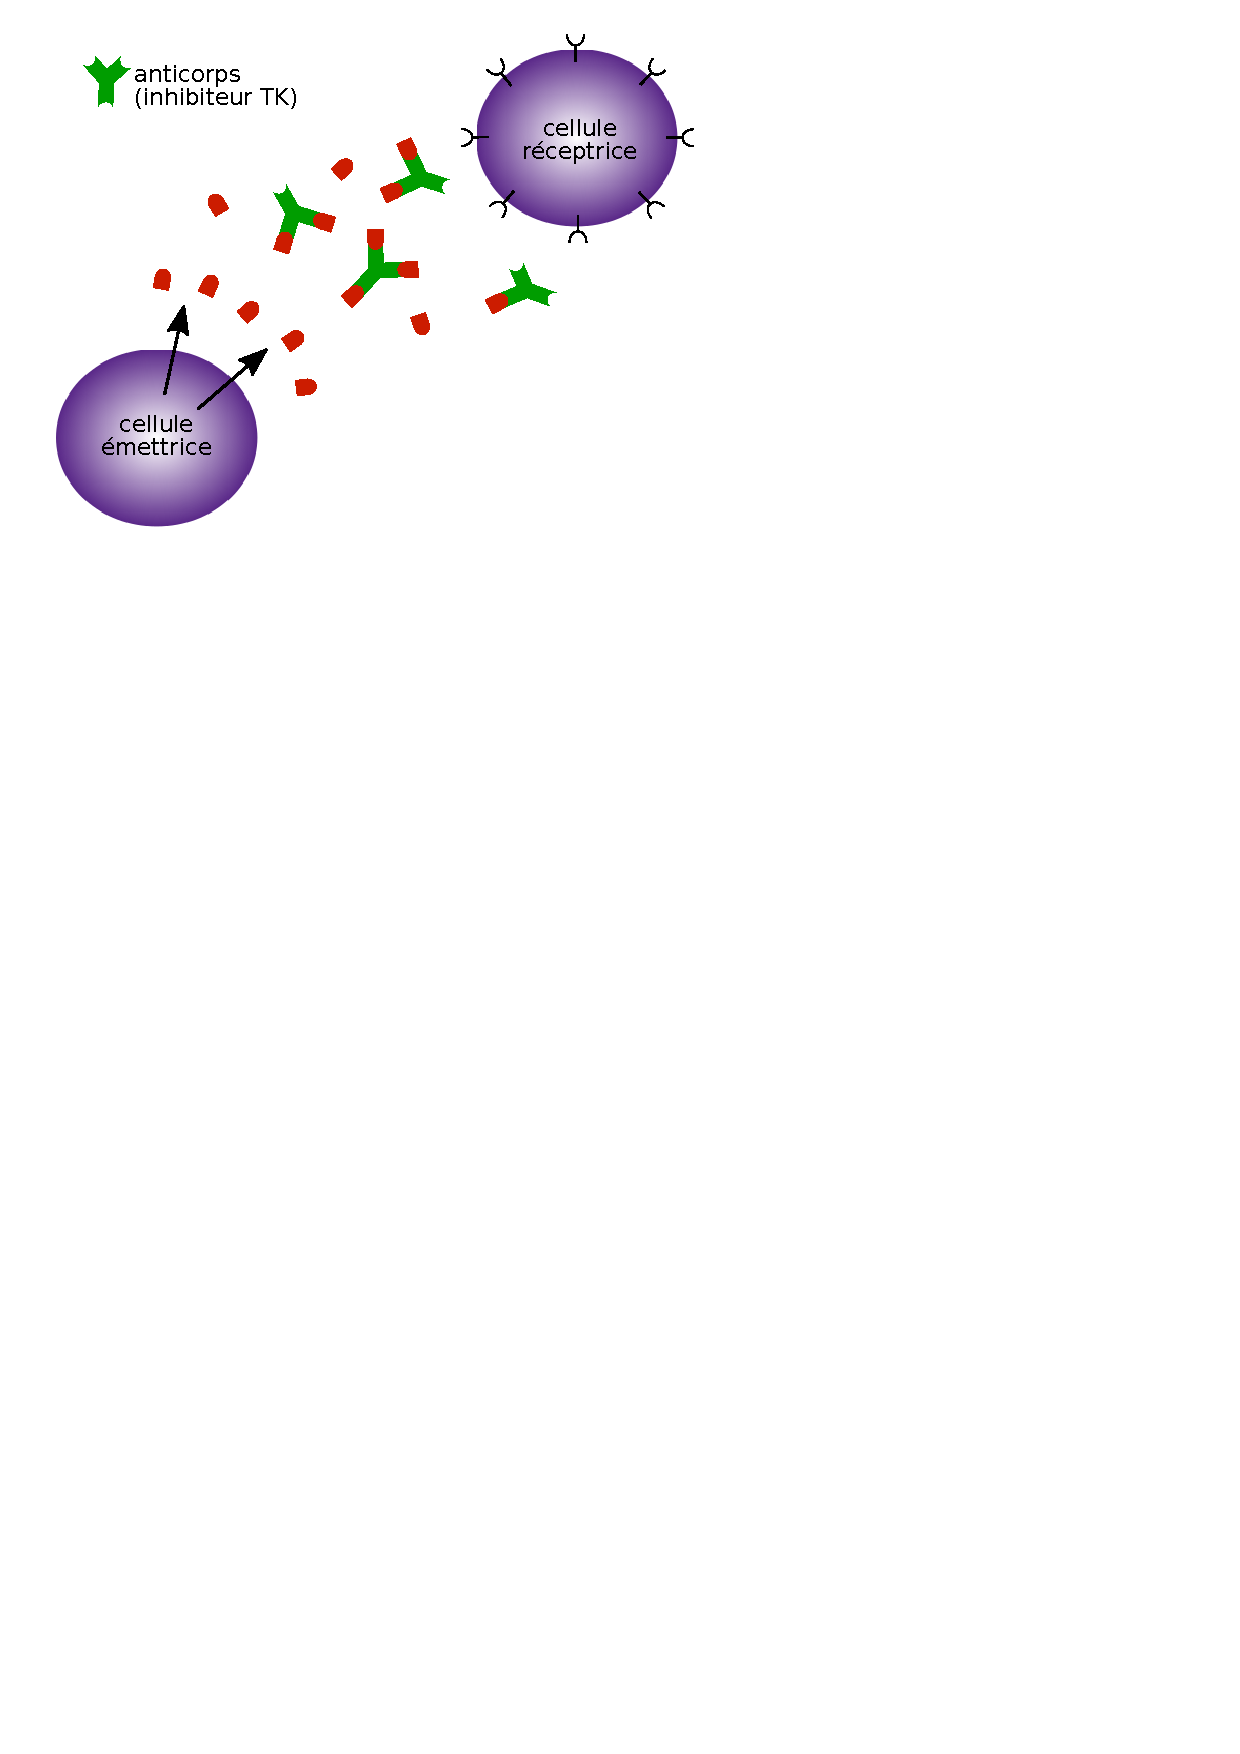
\includegraphics[trim= 0mm 195mm 85mm 0mm, clip=true, width=.32\textwidth]{schema/anticorps.pdf}}\hfill
\subfloat[\label{fig:RTKI}Mode d'action d'un inhibiteur de récepteurs à tyrosine kinase (X-inib)]{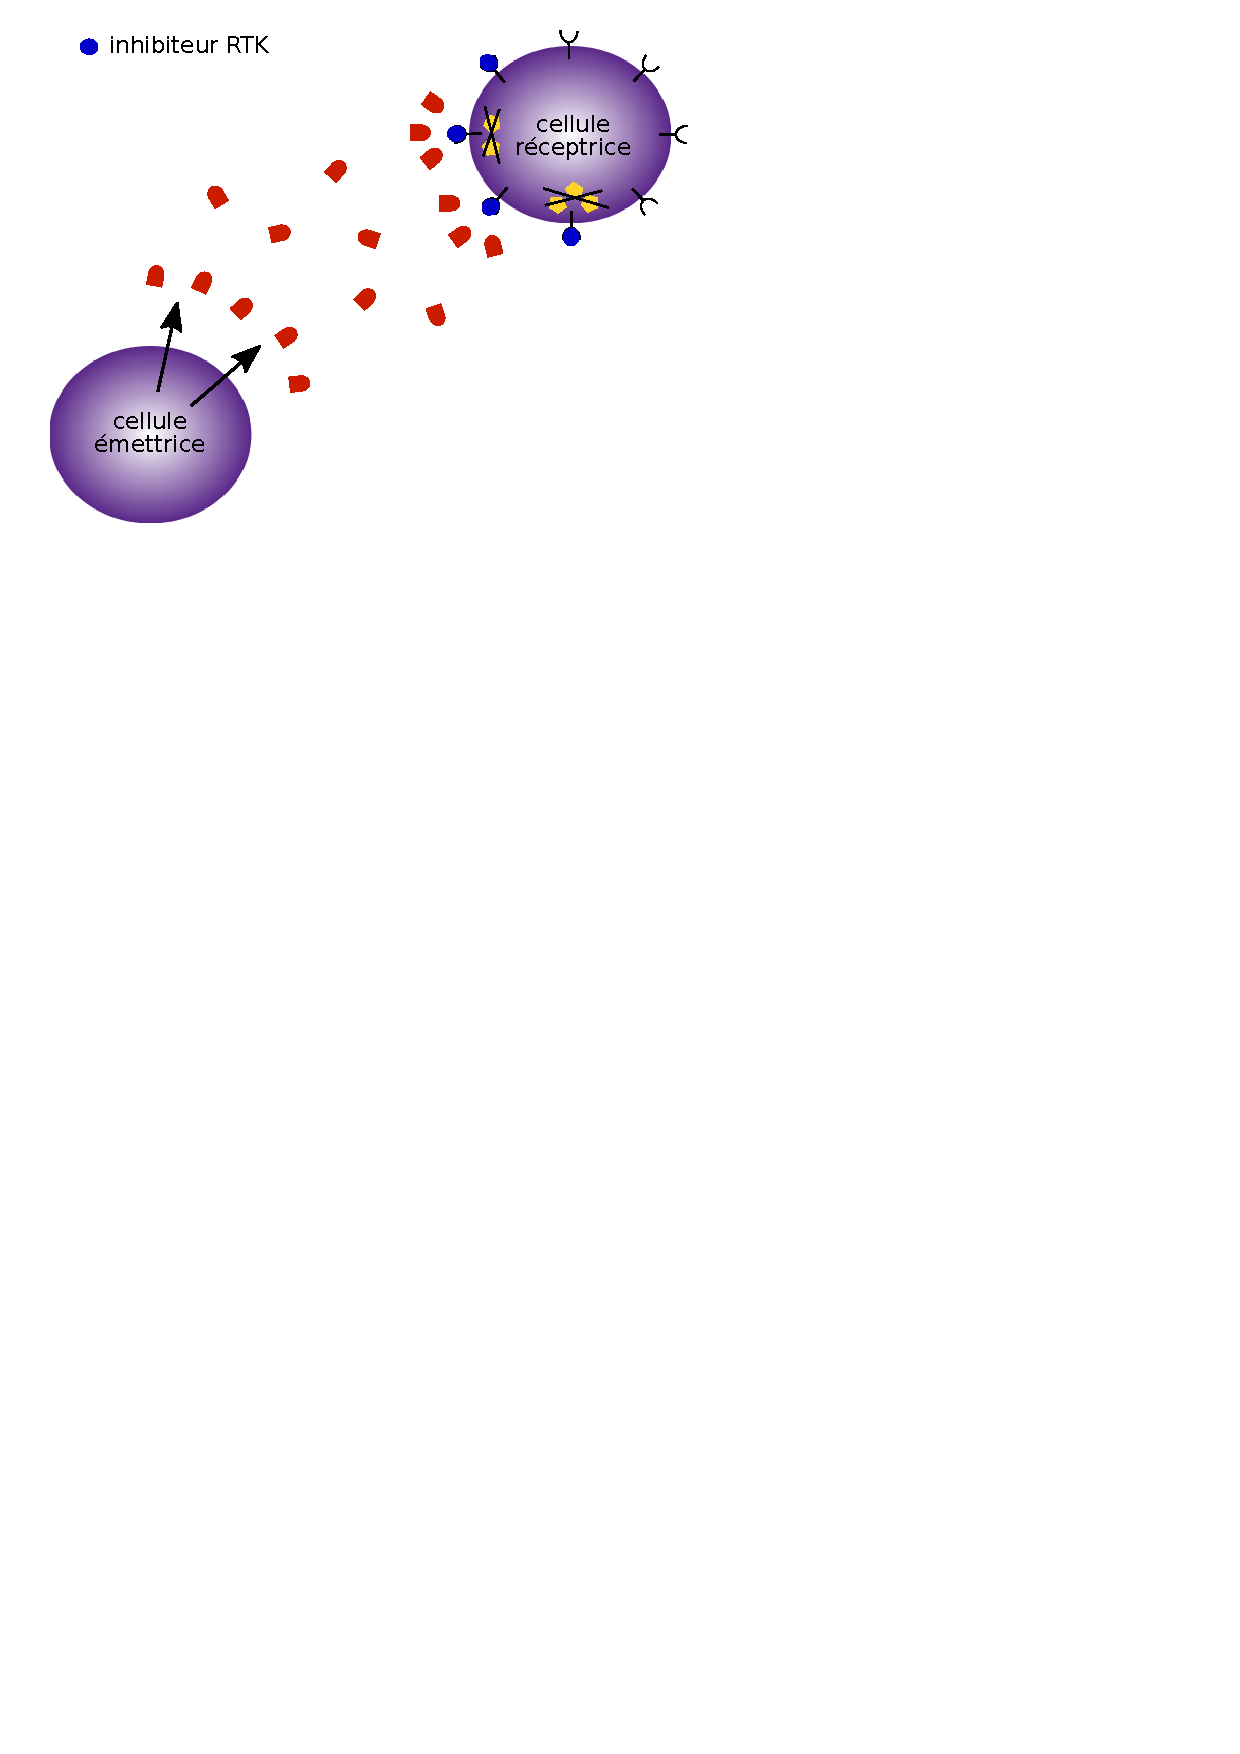
\includegraphics[trim= 0mm 195mm 85mm 0mm, clip=true, width=.32\textwidth]{schema/inhibiteur.pdf}}
\caption{Les tyrosines kinases et leurs inhibiteurs\label{fig:voies_moleculaires}}
\end{figure}

En exemple nous pouvons citer l'\emph{imatinib} (Glivec\footnote{\correction{Nom commercial sous lequel la molécule en question est vendue.\label{footnote:nom_medoc}}}) qui se fixe sur les récepteurs cellulaires de tyrosines kinases %(récepteurs de tyrosine kinase, RTK) 
commandant l'activité intra-cellulaire. En inhibant ces récepteurs, l'apoptose tend à se réactiver dans les cellules défectueuses. 
Nous pouvons également citer le \emph{bévacizumab} (Avastin\samefootnote{footnote:nom_medoc}), qui inhibe l'angiogenèse, en se fixant sur les récepteurs de VEGF (que l'on abrège communément VEGFR). D'autres molécules, comme  le sorafénib ou le sunitinib, ont des effets multiples. 
Le \emph{sorafénib} (Nexavar\samefootnote{footnote:nom_medoc}) est un inhibiteur, à la fois, de VEGFR et de Raf-kinase (tyrosine kinase intervenant dans la cascade de kinases activées lors de la mitose). 
Le \emph{sunitinib} (Sutent\samefootnote{footnote:nom_medoc}) inhibe également les VEGFRs ainsi que les KIT-kinases (protéïnes CD117, qui sont des tyrosines kinases très souvent exprimées dans le cas de GIST, kinases normalement produites uniquement par les cellules souches).
%%\todo[noline]{Kit --> commande la survie, la prolif, ou la division cellulaire}


Tous les cas cliniques que nous étudions dans cet ouvrage ont été traités avec ce type de traitement. Dans le cas de métastases hépatiques de GIST, l'imatinib est recommandé en première ligne~\cite{demetri2002efficacy}. 
%Si 
Lorsque celui-ci devient inefficace %(ce qui arrive très souvent, 
(des cellules résistantes se développant), le sunitinb est utilisé en seconde ligne~\cite{Demetri20061329,saltz2007phase,houk2010relationship}. 
Dans certains cas de mutation génétique (du gène KIT notamment), il a même été montré une résistance à l'imatinib plus accrue que chez les autres patients  (\cf~\cite{rubin2001kit,lux2000kit,lasota2000mutations}).

%============= deb rapportstage M2 ==============\\
%
%\subsubsection{La chimiothérapie}
%La chimiothérapie est l'injection dans le sang d'une substance chimique modifiant la forme de l'ADN de l'ensemble des cellules de l'organisme. Ceci a pour effet que toute cellule voulant se diviser péri. Ceci permet de limiter donc la croissance de la tumeur. Cependant le traitement agit sur toutes les cellules, et donc sur les cellules saines également. Ce qui n'est pas sans laissé d'effets secondaires. L'organisme ne peut plus fabriquer de nouvelle cellules là où il y en a besoin, ce qui se traduit par la perte des cheveux, etc \ldots
%
%\subsubsection{Les anti-angiogéniques}\label{trait antiangio}
%Les anti-angiogénique sont des molécules inhibitrices de l'angiogenèse. Les antiangiogéniques peuvent être classés , selon leur mode d'action, en deux catégories :
%\begin{enumerate}
%\item Les protéïnes se placent sur les récepteurs spécifiques à la VEGF sur les cellules endothéliales, inhibant ainsi l'effet de la VEGF.
%\item Ou bien elles se placent directement sur la VEGF, l'empêchant ainsi de se fixer aux cellules endothéliales.
%\end{enumerate}
% En administrant des anti-angiogénique au patient, on prive alors l'organisme de la création de nouveaux vaisseaux sanguins. La tumeur ne peut alors plus s'alimenter. Ceci n'est pas non plus sans effet secondaires : difficultés de cicatrisation par exemple. Les anti-angiogéniques ont pour effet également de renforcer le réseau sanguin existant. Ceci limite donc la dissémination des métastases par voie sanguine, car celles-ci ont beaucoup plus de mal à entrer dans le réseau.
%
%\subsection{Chimiothérapie et anti-angiogéniques}
%Il s'avère qu'une chimiothérapie seule est assez inefficace. En effet, en grandissant la tumeur détériore le réseau sanguin qui l'alimente. Le traitement arrivant par voie sanguine n'a donc aucune chance d'atteindre le centre de la tumeur. En cumulant chimiothérapie et anti-angiogéniques, le réseau sanguin est consolidé et nettement moins endommagé par la tumeur ce qui permet à la chimiothérapie d'atteindre le c\oe ur de la tumeur et ainsi agir de manière efficace.\\
%=============   FIN RAPPORT STAGE M1  ===========\\

\section{Fonctionnement du scanner \label{sec:fct_scan}}
\subsection{Le scanner en général}
Le scanner est un examen médical qui permet d'acquérir des images d'une partie de l'organisme par le biais d'une irradiation aux rayons~X. %Oui, oui, une irradiation ! 
Cependant l'irradiation est faible et de plus en plus d'études mettent en avant des méthodes pour la réduire encore~\cite{mccollough2009strategies}. Le bénéfice est donc très important devant les risques marginaux. C'est certainement l'une des raisons pour laquelle le scanner (tout comme la radiographie, ou l'IRM) est aujourd'hui très utilisé pour diagnostiquer une maladie, ou %ne serait-ce  que 
pour contrôler la santé d'un patient.


\begin{wrapfigure}[18]{r}{.3\textwidth} %%% L : Left flottant / l: left non flottant (pas de pagebreak)
\vspace{-3mm}
\setlength{\unitlength}{.0032\textwidth}
\begin{picture}(100,121)
\scriptsize
%\footnotesize
\put(0,0){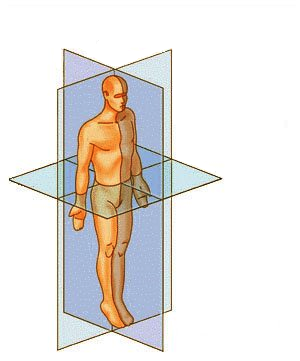
\includegraphics[width=.32\textwidth]{schema/Coupe_anatomie.jpg}}
\put(37,113){\vector(-1,-1){10}}
\put(69,100){\vector(-1,-1){10}}
\put(75,46){\vector(-1,1){10}}
\put(0,115){Plan sagital (ou frontal)}
\put(71,102){Plan}
\put(71,95){coronal}
\put(72,39){Plan}
\put(66,32){axial (ou}
\put(64,25){transverse)}
%%\put(100,0){\line(0,1){121}}
\end{picture}
\captionof{figure}{\label{fig:schema_coupe} Plans de coupe du corps humain.}
\end{wrapfigure}
Un scanner procède par acquisition d'images en couches. En ce qui concerne le scanner du thorax, le patient est \og découpé \fg{} %de part en part 
%% A  voir : http://www.impactscan.org/download/msctdose.pdf
\cite{goldman2008principles} selon le plan axial (\cf Figure~\ref{fig:schema_coupe} présentant l'orientation des plans de coupe). 
Sur chacun de ces plans on mesure l'absorption aux rayons~X~: la \emph{tomodensitométrie}. 
Cette absorption dépend de la densité du tissu mais pas seulement~: elle dépend aussi de sa nature, de sa composition. 
Chaque constituant de l'organisme à sa propre tomodensitométrie. 
Celle-ci se mesure en \emph{unité Hounsfield}~(HU). Sur cette échelle, l'absorption aux rayons~X de l'eau est définie comme étant zéro. Toute autre tomodensitométrie est alors exprimée relativement à cette absorption de référence. Par exemple l'air a une tomodensitométrie de \numprint[HU]{-1000}, le poumon de \numprint[HU]{-500}, la graisse de \numprint{-100} à \numprint[HU]{-50}, le foie autour de \numprint[HU]{+50}, les os entre \numprint{+700} et \numprint[HU]{+3000} %\todo{REF ?} 
selon leur spongiosité. %s'ils sont spongieux ou non. 
La tomodensitométrie est donc très variable. Pour pouvoir visualiser cette quantité, il est nécessaire de choisir une échelle adaptée à ce que l'on veut regarder. L'échelle sera définie par~:
\begin{myitemize}
\item deux absorptions limites choisies. 
Le noir est associé à la plus petite de ces bornes, le blanc à l'autre. Au-delà de ces bornes aucune nuance de couleur n'apparaitra.
\item une fonction qui va définir la manière de passer du noir au blanc. Généralement, une fonction linéaire est considérée \cad que la variation du noir au blanc est constante.
\end{myitemize}
Par exemple, si nous nous intéressons aux poumons, l'échelle pourra être fixée entre \numprint[HU]{-1200} et~\numprint[HU]{+200} (qui est l'échelle suggérée par le logiciel OsiriX~\cite{rosset2004osirix,ratib2006open} dans le cas du poumon). Avec cette échelle le foie apparait tout blanc avec très peu de nuances. Elle est donc inadaptée si nous  souhaitons observer le foie. Pour le foie, une échelle allant de \numprint{-135} à \numprint[HU]{+215} par exemple, sera beaucoup plus adaptée. 
Une telle échelle est illustrée plus loin dans ce manuscrit, \cf Figure~\ref{fig:schema_correspondance_gris} page~\pageref{fig:schema_correspondance_gris}.
Cependant, pour le foie les variations de tomodensitométrie sont assez faibles, même en cas de maladie (métastases notamment). Les médecins ont alors recours à une méthode particulière pour augmenter le contraste des images~: le scanner avec produit de contraste iodé (PCI).


\subsection{Le scanner avec produit de contraste iodé (PCI)}
\begin{figure}[h]
\centering
%%\vspace{-10mm}
\scalebox{.7}{\setlength{\unitlength}{0.01\textwidth}
\begin{picture}(100,100)
\put(0,0){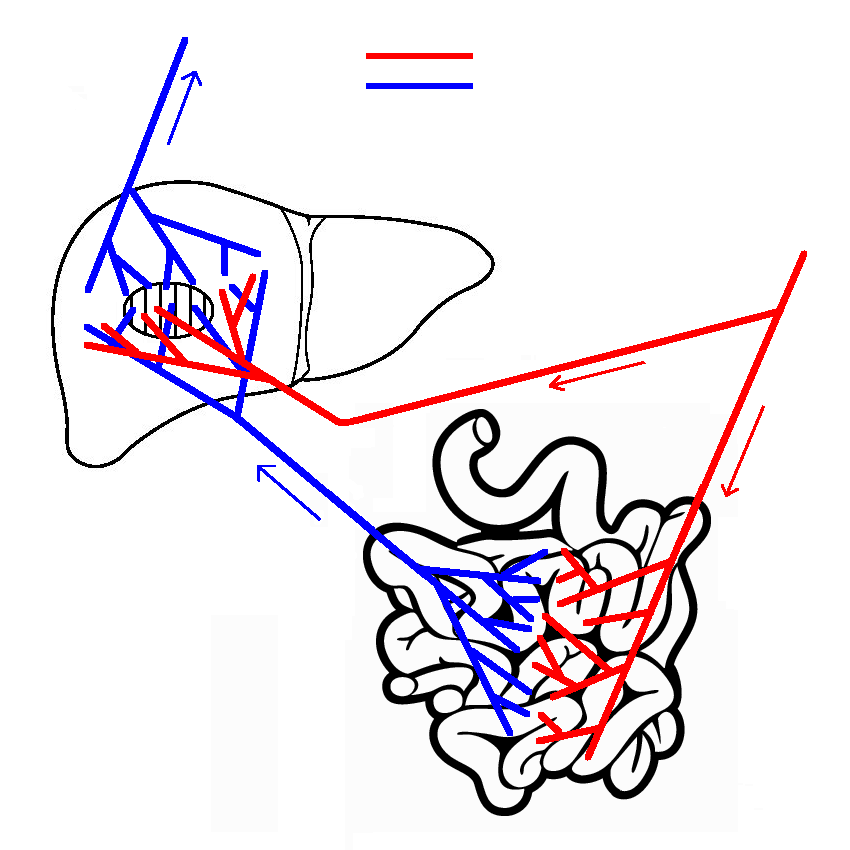
\includegraphics[width=100\unitlength]{schema/schema_irrigation_foie.png}}

%%% Cadre bordure
%\put(0,0){\line(0,1){100}}\put(0,0){\line(1,0){100}}
%\put(100,0){\line(0,1){100}}\put(0,100){\line(1,0){100}}

\put(57,92.5){Sang artériel, riche en oxygène}
\put(57,89){Sang veineux, pauvre en oxygène}

\put(40,75){Foie}
\put(82,18){Intestin grêle}
\put(82,15){et autres}
\put(83,12){organes du}
\put(82,9){tube digestif }

\linethickness{0.4\unitlength}
\put(18,65){\line(-10,-30){10}}
\put(1,32){Métastase}
\put(1,29){hépatique}

\put(57,56){ \begin{turn}{15} Artère hépatique \end{turn} }
\put(11,78){ \begin{turn}{70} Veine hépatique \end{turn} }
\put(31,49){ \begin{turn}{-40} Veine porte \end{turn} }
\put(77.5,48){ \begin{turn}{66} Artère \end{turn} }
\put(79,44){ \begin{turn}{66} mésentérique \end{turn} }
\end{picture}
}
%%\vspace{-10mm}
\caption{\label{fig:schema_irrig_foie} Schéma de l'irrigation du foie.}
\vspace{-3mm}
\end{figure}
%\begin{wrapfigure}[18]{r}{.5\textwidth}
%\scalebox{.5}{\setlength{\unitlength}{0.01\textwidth}
\begin{picture}(100,100)
\put(0,0){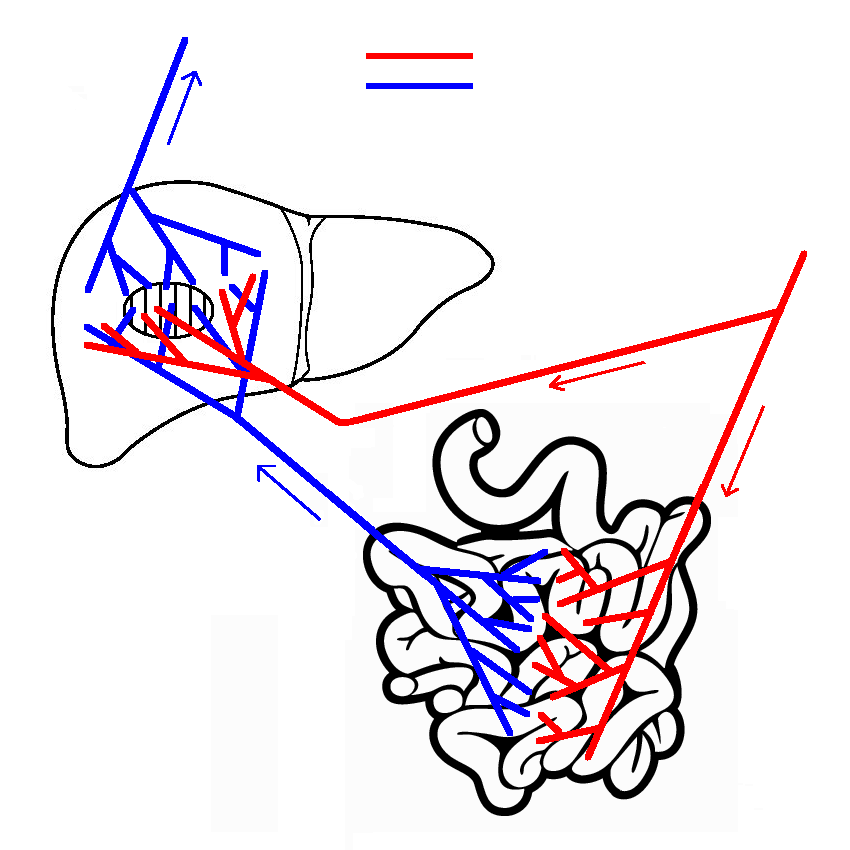
\includegraphics[width=100\unitlength]{schema/schema_irrigation_foie.png}}

%%% Cadre bordure
%\put(0,0){\line(0,1){100}}\put(0,0){\line(1,0){100}}
%\put(100,0){\line(0,1){100}}\put(0,100){\line(1,0){100}}

\put(57,92.5){Sang artériel, riche en oxygène}
\put(57,89){Sang veineux, pauvre en oxygène}

\put(40,75){Foie}
\put(82,18){Intestin grêle}
\put(82,15){et autres}
\put(83,12){organes du}
\put(82,9){tube digestif }

\linethickness{0.4\unitlength}
\put(18,65){\line(-10,-30){10}}
\put(1,32){Métastase}
\put(1,29){hépatique}

\put(57,56){ \begin{turn}{15} Artère hépatique \end{turn} }
\put(11,78){ \begin{turn}{70} Veine hépatique \end{turn} }
\put(31,49){ \begin{turn}{-40} Veine porte \end{turn} }
\put(77.5,48){ \begin{turn}{66} Artère \end{turn} }
\put(79,44){ \begin{turn}{66} mésentérique \end{turn} }
\end{picture}
}
%\vspace{-10mm}
%\caption{\label{fig:schema_irrig_foie} Schéma de l'irrigation du foie.}
%\end{wrapfigure}
Pour réaliser ce type d'examen, la procédure d'acquisition de l'image est la même que pour un simple scanner, avec le même équipement. La différence réside dans l'injection en intraveineuse d'un produit de contraste iodé (PCI), juste avant l'examen~\cite{rengo2011optimal}. 
L'iode ayant un fort taux d'absorption des rayons~X, il va éclaircir l'ensemble des zones dans lequel il se trouve (on appelle ceci le rehaussement). 
En ce qui concerne le foie, pour comprendre pourquoi le foie sain est plus éclairci par le PCI que les métastases, nous devons nous intéresser à la manière dont arrive le PCI au foie et à la tumeur. 
La Figure~\ref{fig:schema_irrig_foie} présente le schéma général de la vascularisation du foie. 
Il possède une double vascularisation. La première est apportée directement depuis le c{\oe}ur par l'artère hépatique. Du sang riche en nutriments (glucose et oygène) vient ainsi irriguer les cellules hépatiques. La seconde provient d'une dérivation. 
Le sang veineux en provenance du système digestif ne retourne pas directement au c{\oe}ur~: il est envoyé au foie par la veine porte. Ce sang bien qu'étant pauvre en oxygène, est riche en glucose puisqu'il contient l'ensemble des éléments digérés. Dans un foie sain, la vascularisation portale est de l'ordre de 70\% et la vascularisation artérielle de l'ordre de 30\%. Dans une tumeur hépatique, ce ratio est inversé~\cite{li2011assessment}. 
En effet, en grandissant la tumeur va accroître ses besoins en glucose mais aussi en oxygène~: la néovascularisation se fait donc principalement depuis la vascularisation artérielle. 


Revenons au PCI. Dans la mesure où il y a deux voies sanguines pour accéder au foie, il y a deux temps caractéristiques~(\cf~\cite{kim2014ct,ichikawa2006multiphasic}):
\begin{myitemize}
\item Le \emph{temps artériel.} C'est le temps après l'injection, que le PCI met pour parvenir au foie par la voie artérielle. Il est d'environ 30 secondes.
\item Le \emph{temps portal.} C'est le temps après l'injection, que le PCI met pour parvenir au foie par la voie portale. Il est d'environ 70 secondes. 
\end{myitemize}
Les scanners réalisés avec PCI, sont effectués au temps portal. Ainsi au moment de l'acquisition de l'image, le PCI se trouve majoritairement dans les tissus vascularisés par la voie portale \ie le foie sain. Le tissu tumoral, beaucoup moins irrigué par voie portale contiendra donc nettement moins de PCI. Ceci se traduit directement sur le contraste de l'image médicale~: le tissu sain ayant fortement éclairci, le tissu tumoral apparait de manière beaucoup plus évidente, en sombre. 
%On pourra même distinguer 
Des nuances au sein de la tumeur (entre le centre et le pourtour notamment) seront même discernables, ce qui va particulièrement nous intéresser pour tout ce qui concerne l'\hetero tumorale. L'ensemble des scanners présentés dans cet ouvrage a été réalisé avec un PCI.

\section{Evaluation clinique de la réponse au traitement~: le critère RECIST}
La surveillance des patients ayant des métastases hépatiques de GIST est assurée grâce à des scanners avec PCI réalisés environ tous les 2 mois. Ainsi, tous les 2 mois, les médecins acquièrent une série d'images en niveaux de gris, chaque image représentant une coupe transversale du thorax du patient. Les images que nous possédons ont une résolution de $512\times512$ pixels et chaque image est espacée d'environ \numprint[mm]{1}, ce qui représente environ 800 images par scanner du thorax. 
Le foie est présent sur environ 200 de ces coupes. 
Ceci représente donc un nombre important de pixels. 
Ainsi, pour évaluer la progression de la tumeur, il est nécessaire d'avoir un critère, qui permette de synthétiser les informations apportées par tous ces nombreux pixels. 
Le critère RECIST (de l'anglais Response Evaluation Criteria In Solid Tumors) est actuellement utilisé. 
Il consiste à ne retenir de chaque scanner qu'une seule et unique information~: le diamètre de la métastase (ou de la plus grosse des métastases si le patient en a plusieurs). Si ce diamètre décroît ou est stable, alors le traitement est considéré comme efficace. S'il augmente de plus de 10\,\%, %alors
 l'échec thérapeutique est considéré %(et dans ce cas là, 
 (le traitement est alors changé). 
 Ce critère a l'avantage d'être simple. 
Ceci étant, il a déjà démontré ses limites~\cite{benjamin2007we,choi2007correlation}, principalement dans l'évaluation de l'efficacité de traitements antiangiogéniques qui font apparaître  beaucoup de nécrose. 
D'autres critères sont à l'étude, dont le critère Choi notamment  (\cf~\cite{choi2008response,kalkmann2012consensus}). 
%, qui prend en compte aussi les densités internes de la métastase. 
\correction{Ce critère améliore le critère RECIST. Il tient compte du diamètre de la métastase mais aussi de son niveau de gris moyen. Il illustre notamment qu'une tumeur peut évoluer sans qu'il y ait nécessairement une variation de l'aire tumorale~: dans ce cas les densités tumorales (et donc le  niveau de gris sur le scanner) varient. 
Les travaux présentés ici, proposent une manière plus fine d'examiner les niveaux de gris par la prise en compte de leur répartition spatiale.}

Dans le chapitre suivant, nous allons construire un modèle mathématique qui simule la croissance d'une tumeur. Ce modèle qui se démarque des précédents modèles notamment par son caractère spatial, soulignera particulièrement l'importance de la prise en compte des densités (caractère homogène ou \heterogene) dans l'évaluation de la réponse aux traitements dans le cas de métastases hépatiques de GIST.

\section{Métastases hépatiques de GISTs}
Les tumeurs stromales gastro-intestinales (GISTs) sont les plus communes de toutes les tumeurs 
gastro-intestinales non épithéliales. Elles ont une incidence de 9 à 14 cas par million de personnes par an (\cf~\cite{Nilsson2005}). 
Dans 25\% des cas (\cf~\cite{dematteo2000}), ce type 
de cancer migre au foie. 


Bien que les GISTs résistent à la plupart des chimiothérapies anticancéreuses conventionnelles~\cite{demetri2011gastrointestinal}, 
la découverte de mutations actives du gène KIT, aussi bien que le rôle du PDGFR\footnote{un type particulier de récepteurs de facteurs de croissances. De l'anglais~: Platelet Derived Growth Factor Receptor} et le développement thérapeutique qui en découle, ont révolutionné le traitement des GISTs.
%the discovery of activating mutations of the KIT as well as the role of PDGFR and the new subsequent therapeutic development have revolutionized GISTs traitements. 
Grâce à ces thérapies ciblées, les GISTs sont devenus des modèles typiques de traitements personnalisés du cancer~\cite{Blay2012}. 
En particulier, la vie des patients ayant un GIST a été améliorée avec l'utilisation d'inhibiteurs de tyrosine kinase comme l'imatinib en première ligne, puis avec un inhibiteur multi-récepteurs de tyrosine kinase comme 
le sunitinib ou le sorafénib,  
qui inhibe les PDGFRs, VEGFRs et KIT, en seconde ligne de traitement. 
Cependant plusieurs limites, en terme de diagnostic et en terme de résultats, résident encore.
% However several limitations in terms of diagnosis and outcomes still remain. 
Tout d'abord, une importante variabilité existe dans les caractéristiques moléculaires et génétiques qui gouvernent le pathogène de ces tumeurs.
Hirota \etal\ ont démontré la présence d'altérations moléculaires du gène KIT dans ces tumeurs (\cf \cite{Hirota1998}). 
En plus de ces mutations de la tumeur primaire, de secondes mutations ont été identifiées chez les patients atteints de GIST avancé prétraité avec un inhibiteur de tyrosine kinase. A l'heure actuelle, 10 ensembles moléculaires différents de GIST avec différentes altérations moléculaires ont été identifiés. 
Chez les patients avec une mutation du gène KIT, une résistance à l'imatinib est fréquemment observée, comme reporté dans~\cite{Blay2011} et montré sur la Figure~\ref{fig:patients_EXON_a}. 
\correction{Dans ces cas là, il est alors fréquent de démarrer directement avec un traitement habituellement administré en seconde ligne (\cf Figure~\ref{fig:patients_EXON_b}).}  
Chez les autres patients, l'imatinib contrôle les lésions métastatiques pendant une période plus ou moins longue, autour de~20-24 mois dans~85\% des cas. 
Les praticiens doivent ensuite changer de molécule, ou bien utiliser une thérapie alternative. 
Comme le pronostic et la sensibilité aux thérapies ciblées dépendent de chaque patient, notre but est de développer un modèle mathématique qui soit basé sur les images médicales des métastases au foie et qui soit dépendant de chaque patient. 
Nous nous intéressons ici aux GISTs avancés afin de déterminer, pour chaque patient, aussi bien le moment de l'émergence de mutations dans les cellules cancéreuses, que le temps de rechute après la première ligne et la seconde ligne de traitement ainsi que des aspects géométriques de la croissance tumorale.

\begin{figure}
\subfloat[Patient présentant une mutation génétique EXON 11\label{fig:patients_EXON_a}]{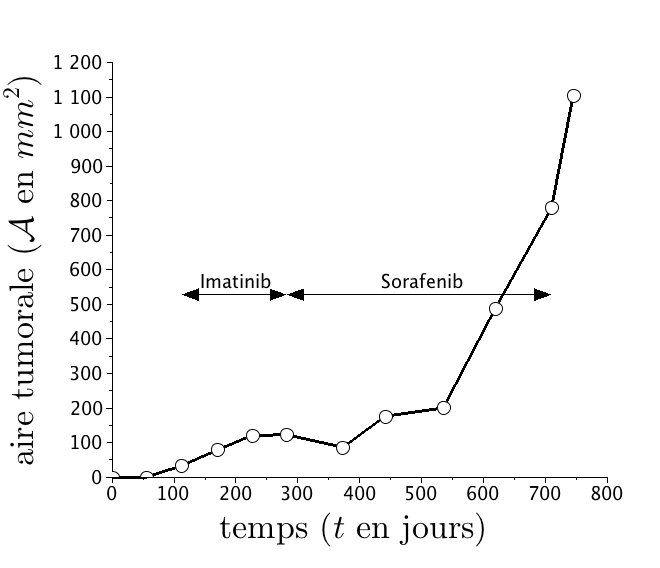
\includegraphics[width=.48\textwidth]{brio.png}}\hfill
\subfloat[Patient présentant une mutation génétique EXON 9\label{fig:patients_EXON_b}]{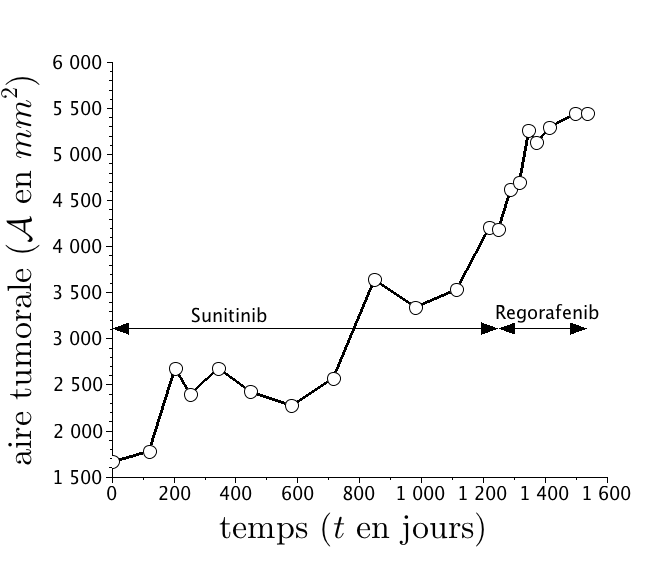
\includegraphics[width=.48\textwidth]{LAN.png}}
\caption{\label{fig:patients_EXON}Evolution de l'aire tumorale sur deux patients présentant des mutations génétiques EXON -- De telles mutations engendrent des résistances aux traitements accrues.}
\end{figure}


Ensuite, les nouveaux agents anti-cancéreux avec des mécanismes d'actions ciblés, comme ceux utilisés pour traiter les GISTs, ont démontré les limitations inhérentes et l'inadéquation de  l'évaluation usuelle (\ie le critère RECIST, \cf~\cite{suzuki2008}) de l'anatomie tumorale. En effet, celle-ci ne considère seulement que le plus large diamètre de la lésion. 
Pour les cliniciens, le challenge consiste à optimiser ces traitements et en particulier à déterminer le moment le plus adéquat pour passer de la première ligne de traitement à la seconde afin d'augmenter la survie globale du patient. L'estimation du temps de rechute est donc cruciale.


Pour surveiller l'évolution de la maladie, le suivi clinique est principalement réalisé avec des scanners. 
Nous soulignons que l'effet de ces nouveaux médicaments change le paradigme selon lequel la sensibilité de la tumeur au traitement est mesurée (\cf \cite{schramm2013}), car les scanners montrent d'autres informations comme l'hétérogénéité tumorale~: le critère RECIST ne semble plus suffisant.

\end{document}